\begin{problem}
  {Q3(a)}
  List all the minimum $s-t$ cuts in the flow network in figure 7.24 (reproduced below).
  \begin{center}
  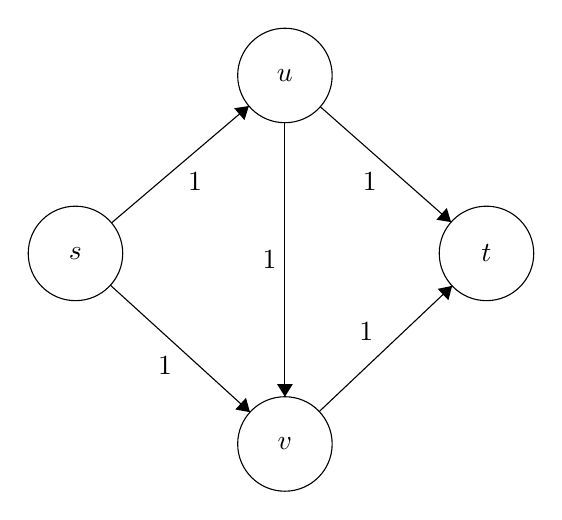
\begin{tikzpicture}[scale=0.2]
  \tikzstyle{every node}+=[inner sep=0pt]
  \draw [black] (21,-27.8) circle (3);
  \draw (21,-27.8) node {$s$};
  \draw [black] (34.3,-16.5) circle (3);
  \draw (34.3,-16.5) node {$u$};
  \draw [black] (34.3,-39.9) circle (3);
  \draw (34.3,-39.9) node {$v$};
  \draw [black] (47.1,-27.8) circle (3);
  \draw (47.1,-27.8) node {$t$};
  \draw [black] (23.29,-25.86) -- (32.01,-18.44);
  \fill [black] (32.01,-18.44) -- (31.08,-18.58) -- (31.73,-19.34);
  \draw (28.6,-22.64) node [below] {$1$};
  \draw [black] (23.22,-29.82) -- (32.08,-37.88);
  \fill [black] (32.08,-37.88) -- (31.83,-36.97) -- (31.15,-37.71);
  \draw (26.69,-34.34) node [below] {$1$};
  \draw [black] (34.3,-19.5) -- (34.3,-36.9);
  \fill [black] (34.3,-36.9) -- (34.8,-36.1) -- (33.8,-36.1);
  \draw (33.8,-28.2) node [left] {$1$};
  \draw [black] (36.48,-37.84) -- (44.92,-29.86);
  \fill [black] (44.92,-29.86) -- (44,-30.05) -- (44.68,-30.77);
  \draw (39.46,-33.37) node [above] {$1$};
  \draw [black] (36.55,-18.49) -- (44.85,-25.81);
  \fill [black] (44.85,-25.81) -- (44.58,-24.91) -- (43.92,-25.66);
  \draw (39.69,-22.64) node [below] {$1$};
  \end{tikzpicture}
  \end{center}
  \noindent
  \textbf{Minimum cuts:}
  \begin{enumerate}
    \item $\{s\}, \{u,v,t\}$
    \item $\{s,v\}, \{u,t\}$
    \item $\{s,v,u\}, \{t\}$
  \end{enumerate}
\end{problem}
